\begin{itemize}

    \item We should have videos or worksheets for the math behind some of the concepts such as partial fractions, integrals, etc.
    \item Try doing more circuit examples.
    \item Keep notation consistent throughout the course...
    \item I like how the book will introduce a concept, do examples, and then give ways to visualize or solve the problems in matlab. We should try doing that more in hw's or exercises and say hey! try this yourself and mess with it.
    \item What is the order idea: Discrete vs. Continuous, what first? Or both at the same time?
\end{itemize}


\subsection{Peter's Notes}
\begin{itemize}
    \item Time invariance could be taught better with more examples. More graphical intuition.
    \item Stability was not made clear. 
    \item Have videos or text with the required math for the class (i.e. differential equations, partial fractions).
\end{itemize}

\subsection{Day by Day}

\begin{center}
    \begin{tabular}{ |c|c| } 
     \hline
     Day1 & Intro to Course + Basic Signals \\ 
     \hline
     Day2 & Impulse Function, Unit Step, Impulse response \\ 
     \hline
     Day3 & Systems + Properties \\ 
     \hline
     Day5 & Discrete Time Convolution \\ 
     \hline
     Day6 & Continuous Time Convolution \\ 
     \hline
     Day7 & Differential Equations\\ 
     \hline
     Day8 & Difference Equations \\ 
     \hline
    \end{tabular}
    \end{center}

\subsection{Student Questions/Comments}
\begin{example}
I've heard from multiple people that time invariance (and properties in general) need to be exampled a lot better considering how important they are in the course.
\begin{center}
    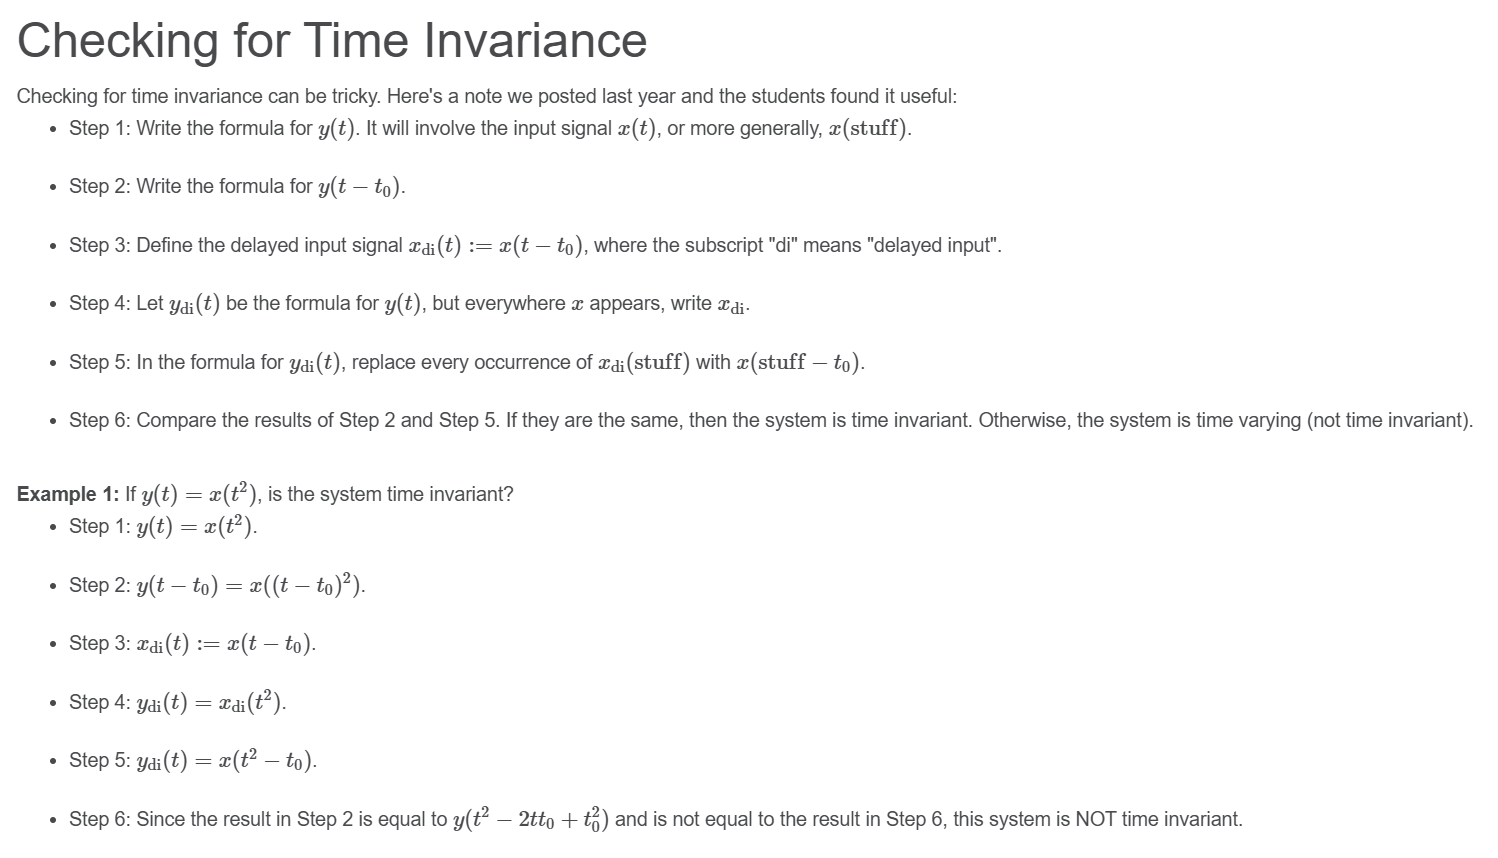
\includegraphics[width = 0.6\textwidth]{images/checking_for_time_invariance.png}       
\end{center}
\end{example}

\begin{itemize}
    \item How to know if something is BIBO stable? Considering it is the first question on the exam, it should be clear to students the steps.
    \item 
\end{itemize}

